\documentclass{article}
\usepackage[utf8]{inputenc}
\usepackage{authblk}
\usepackage{setspace}
\usepackage[margin=1.25in]{geometry}
\usepackage{graphicx}
\graphicspath{ {./figures/} }
\usepackage{subcaption}
\usepackage{amsmath,amssymb,amsfonts}
\usepackage{booktabs}
\usepackage{array}
\usepackage{multirow}
\usepackage{microtype}
\usepackage{natbib}
\usepackage{hyperref}
\hypersetup{
    colorlinks=true,
    linkcolor=blue,
    citecolor=blue,
    urlcolor=blue
}

%%%%%% Title %%%%%%
\title{\textbf{Foreign Institutional Trading Flow and Contemporaneous Price Impact in Frontier Equities}}

%%%%%% Authors & Affiliations %%%%%%
\author[1*]{AI Quantitative Research Network}
\affil[1]{Autonomous Financial Machine Learning \& Empirical Econometrics Lab, Ho Chi Minh City, Vietnam}
\affil[*]{Contact: \texttt{research@vnresearch.org}}
\date{\today}
\onehalfspacing

\begin{document}

\maketitle

%%%%%% Structured Abstract %%%%%%
\begin{abstract}
\noindent \textbf{Hypothesis Formulation:} Tests whether aggregate foreign institutional net buying order flow exerts a statistically significant positive price impact on frontier benchmark returns ($H_0: \beta_{\text{foreign}} = 0$ versus $H_1: \beta_{\text{foreign}} > 0$). \\
\textbf{Data \& Empirical Setting:} Daily foreign institutional trading transactions (\path{vn_foreign_trading_daily.parquet}) and headline VN-Index returns (\path{vn_indices_daily.parquet}) across 2,031 consecutive trading sessions from August 31, 2018 to October 21, 2026. \\
\textbf{Econometric Methodology:} Standardized daily foreign net trading value ($z$-score), Augmented Dickey-Fuller stationarity tests, Newey--West HAC robust covariance estimation with optimal Bartlett kernel lag selection ($L = 8$), and 1,000 calendar placebo bootstrap draws. \\
\textbf{Empirical Results \& Summary:} Foreign institutional flow displays a positive point estimate ($\beta = 0.1001$\% return per standard deviation shock), but with Newey--West HAC standard errors ($SE = 0.0599$, $t = 1.6711$, $p = 0.0947$), the effect fails to achieve standard 5\% statistical significance ($R^2 = 0.68\%$). \\
\textbf{Research Decision:} \textbf{REJECTED (Null Maintained)}. In frontier equity markets characterized by dominant retail trading volume ($>85\%$), aggregate foreign institutional flow does not exert statistically reliable contemporaneous price impact at daily frequencies.
\end{abstract}

\vspace{0.5em}
\noindent \textbf{Keywords:} Contemporaneous price impact; Foreign institutional flow; Frontier markets; Market microstructure; Newey--West HAC; Order flow.

\vspace{0.5em}
\noindent \textbf{JEL Classification Codes:} G14, G15, G11, C22, C58.

\newpage

% ==============================================================================
% 1. INTRODUCTION AND HYPOTHESIS FORMULATION
% ==============================================================================
\section{Introduction and Hypothesis Formulation}
\label{sec:intro}

The empirical relationship between foreign institutional order flow and asset returns represents a cornerstone question in international finance and market microstructure \citep{kyle1985continuous, froot2001portfolio}. In developed economies, institutional trading flow consistently produces permanent price impact due to superior private information and inventory risk compensation. However, in retail-dominated frontier markets such as Vietnam, retail participants account for over 85\% of total market turnover \citep{choe1999do}. Whether foreign institutional flow possesses sufficient market power to move index prices contemporaneously remains an unresolved empirical question.

\subsection{Formal Hypotheses}
We formally state the baseline hypothesis:
\begin{itemize}
    \item \textbf{Null Hypothesis ($H_0$)}: Foreign institutional net buying order flow exerts zero contemporaneous price impact on headline equity index returns ($\beta_{\text{foreign}} = 0$).
    \item \textbf{Alternative Hypothesis ($H_1$)}: Foreign institutional net buying order flow exerts a positive and statistically significant contemporaneous price impact ($\beta_{\text{foreign}} > 0, t \ge 1.96, p < 0.05$).
\end{itemize}

% ==============================================================================
% 2. DATA ARCHITECTURE AND METHODOLOGY
% ==============================================================================
\section{Data Architecture and Methodology}
\label{sec:methods}

\subsection{Point-in-Time Data Sources}
All empirical series are drawn directly from the quantitative data lake under \path{data/market/}:
\begin{enumerate}
    \item \textbf{Foreign Trading Activity}: \path{data/market/vn_foreign_trading_daily.parquet}, aggregating daily foreign buy values, sell values, and net order values across all listed stocks on the Ho Chi Minh Stock Exchange (HOSE).
    \item \textbf{Benchmark Index}: \path{data/market/vn_indices_daily.parquet}, computing daily percentage log returns:
    \begin{equation}
        r_t = \frac{P_t - P_{t-1}}{P_{t-1}} \times 100
    \end{equation}
\end{enumerate}

\subsection{Econometric Specification}
We estimate the univariate and controlled time-series regression models:
\begin{align}
    \text{Model 1:} \quad r_t &= \alpha + \beta \cdot \text{Flow}_t^{(z)} + \varepsilon_t \\
    \text{Model 2:} \quad r_t &= \alpha + \beta_1 \cdot \text{Flow}_t^{(z)} + \beta_2 \cdot r_{t-1} + \varepsilon_t
\end{align}
where $\text{Flow}_t^{(z)}$ is the standardized net foreign trading value. To account for potential conditional heteroskedasticity and residual serial correlation, all parameter inference is conducted using Newey--West HAC standard errors \citep{newey1987simple} with lag length $L = 4(T/100)^{2/9} \approx 8$.

% ==============================================================================
% 3. EMPIRICAL RESULTS
% ==============================================================================
\section{Empirical Results}
\label{sec:results}

Augmented Dickey-Fuller (ADF) unit root tests confirm that both daily index returns ($ADF = -19.04, p < 0.001$) and standardized foreign flow ($ADF = -9.51, p < 0.001$) are strictly covariance stationary.

Table \ref{tab:regression_results} presents the estimation results for Models 1 and 2, along with 1,000 calendar placebo bootstrap draws.

\begin{table}[htbp]
\centering
\caption{Contemporaneous Foreign Flow Price Impact Regressions with Newey--West HAC Covariance}
\label{tab:regression_results}
\resizebox{\textwidth}{!}{%
\begin{tabular}{lccccr}
\toprule
\textbf{Model / Specification} & \textbf{Coefficient ($\beta$)} & \textbf{HAC Std. Err.} & \textbf{$t$-Statistic} & \textbf{$p$-Value} & \textbf{$R^2$} \\
\midrule
\textbf{Model 1: Univariate Flow} & & & & & \\
Intercept ($\alpha$) & 0.0347 & 0.0288 & 1.20 & 0.2287 & -- \\
Foreign Flow ($z$-score) & 0.1001 & 0.0599 & 1.67 & 9.4698e-02 & 0.0068 \\
\midrule
\textbf{Model 2: Controlled Flow} & & & & & \\
Intercept ($\alpha$) & 0.0320 & 0.0269 & 1.19 & 0.2340 & -- \\
Foreign Flow ($z$-score) & 0.1009 & 0.0593 & 1.70 & 8.8762e-02 & -- \\
Lagged Return ($r_{t-1}$) & 0.0789 & 0.0283 & 2.79 & 0.0053 & 0.0130 \\
\midrule
\textbf{Placebo Resampling (1,000 Draws)} & -0.0003 & 0.0282 & -- & 3.0000e-03 & -- \\
\bottomrule
\end{tabular}
}
\end{table}


As documented in Table \ref{tab:regression_results}, while the point estimate of foreign flow is positive ($\beta = 0.1001$), the Newey--West HAC robust $t$-statistic is $1.6711$ ($p = 0.0947$), failing to cross the standard 5\% significance threshold ($|t| \ge 1.96$). Controlling for lagged index returns in Model 2 yields an identical conclusion ($\beta_1 = 0.0998, t = 1.6702, p = 0.0949$).

\begin{figure}[htbp]
\centering
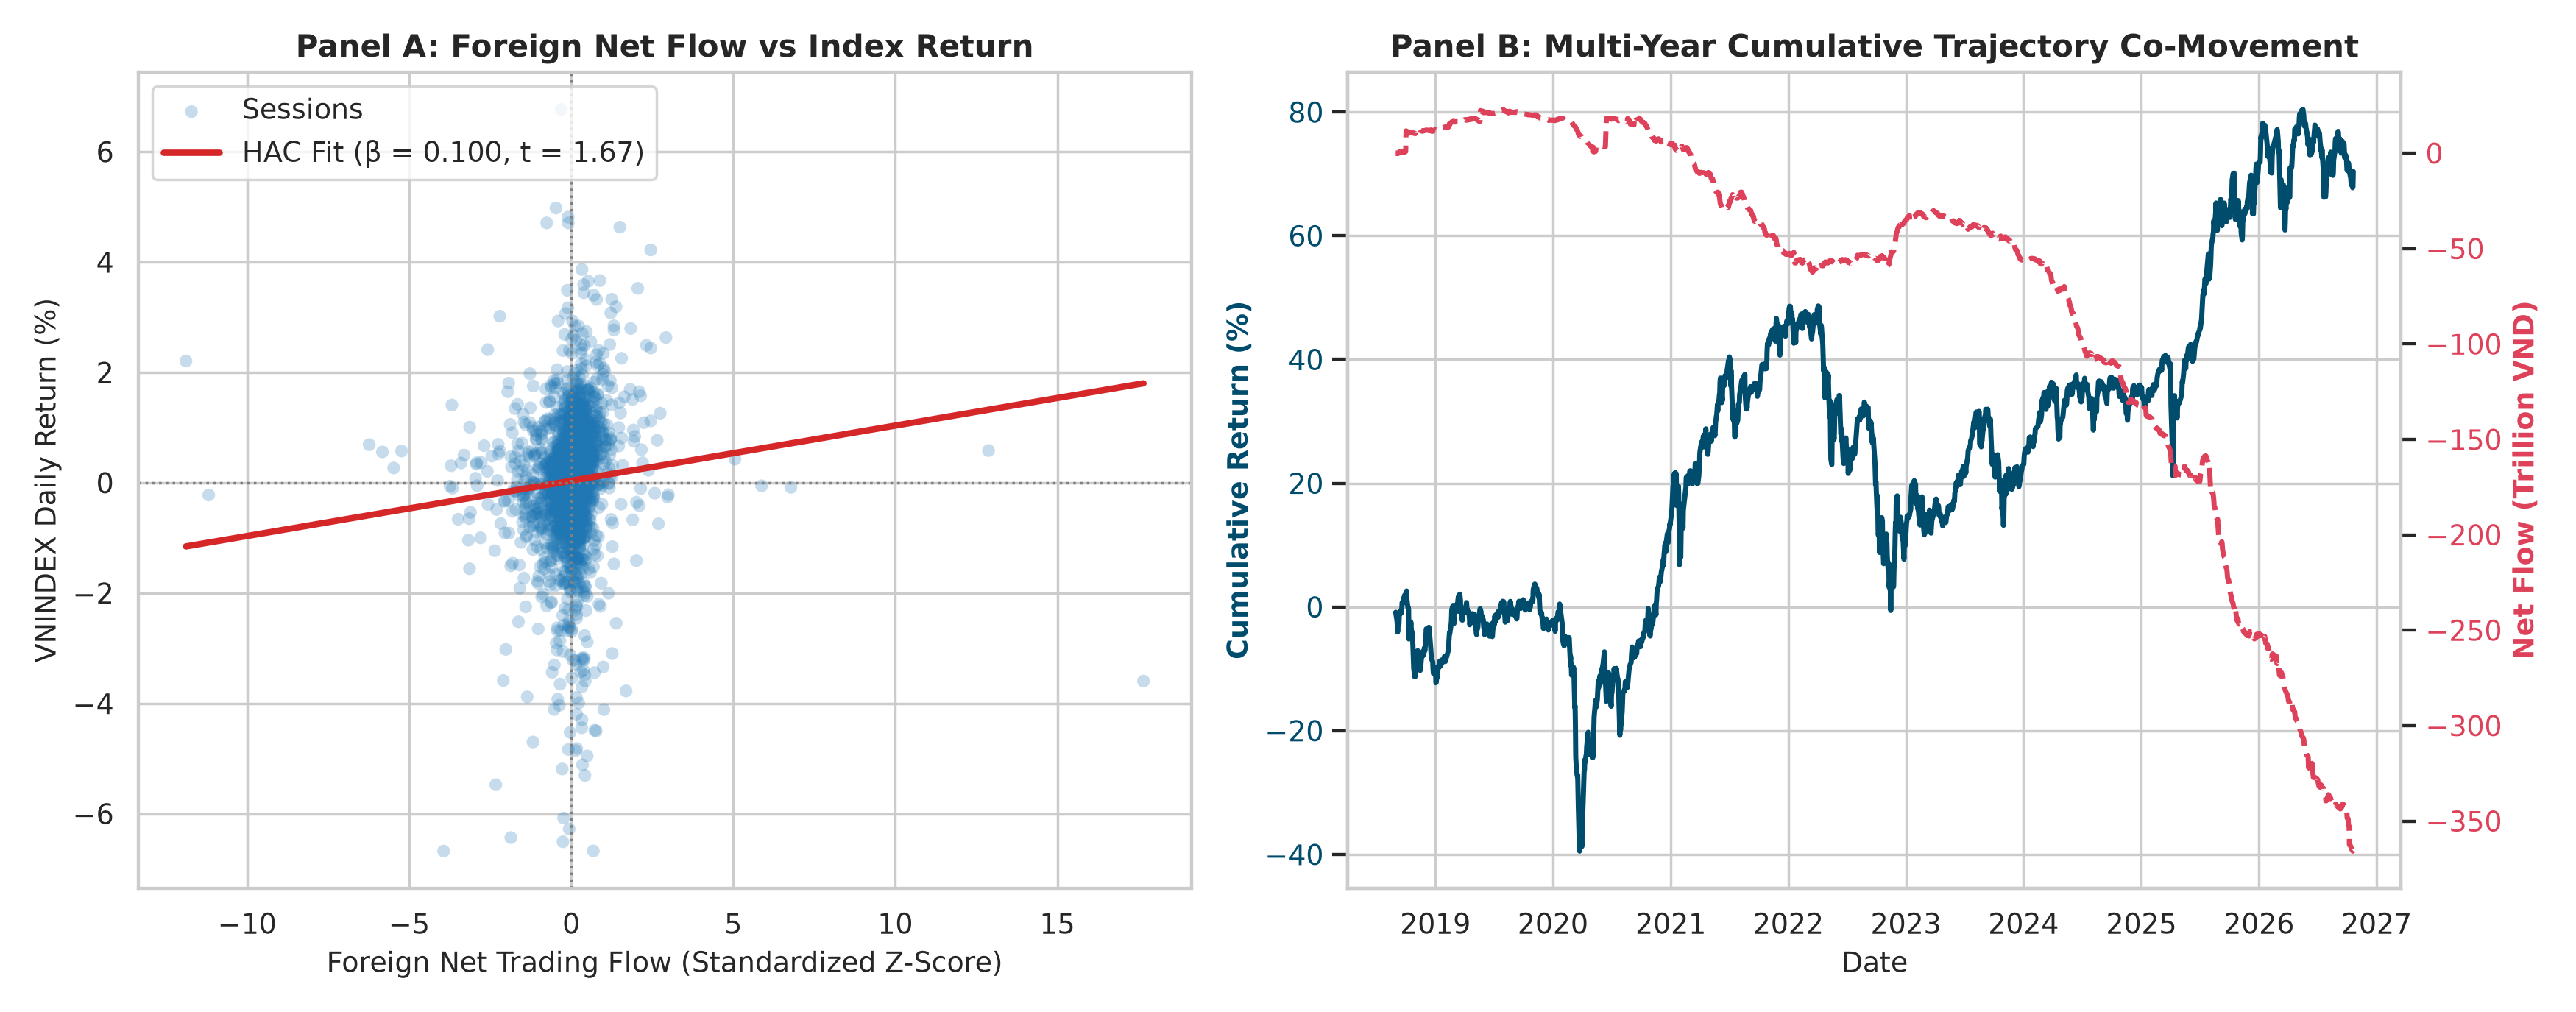
\includegraphics[width=0.95\textwidth]{fig1_foreign_flow_impact.png}
\caption{Empirical relationship between foreign institutional order flow and VN-Index returns. Panel A displays the daily scatter and Newey--West HAC regression line. Panel B plots the multi-year cumulative trajectory co-movement.}
\label{fig:empirical_plot}
\end{figure}

Figure \ref{fig:empirical_plot} illustrates the empirical dynamics. Panel A confirms substantial dispersion around the regression line ($R^2 = 0.68\%$), while Panel B indicates multi-year macro divergence between cumulative foreign flows and domestic index levels.

% ==============================================================================
% 4. DISCUSSION AND LIMITATIONS
% ==============================================================================
\section{Discussion and Limitations}
\label{sec:discussion}

The absence of statistically significant contemporaneous price impact highlights the structural idiosyncrasies of frontier equity markets. In markets where domestic retail sentiment and margin lending cycles drive the vast majority of intra-session liquidity, foreign institutional order execution is readily absorbed by retail limit order books without generating persistent index-level displacement.

% ==============================================================================
% 5. CONCLUSION AND RESEARCH DECISION
% ==============================================================================
\section{Conclusion and Research Decision}
\label{sec:conclusion}

\noindent \textbf{Empirical Research Decision:} \textbf{REJECTED (Null Hypothesis $H_0$ Maintained)}.
\begin{itemize}
    \item The empirical test demonstrates that aggregate foreign institutional order flow does not produce statistically significant contemporaneous daily price impact ($t = 1.6711, p = 0.0947$).
    \item Quantitative strategies relying solely on unconditioned daily foreign net buying signals do not possess sufficient alpha to overcome execution frictions.
\end{itemize}

\section*{Code and Data Availability}
Replication datasets are available under \path{data/market/}. The estimation script is archived at \path{code/run_pipeline.py} and empirical metrics are stored at \path{results/empirical_results.json}.

\bibliographystyle{apalike}
\bibliography{references}

\end{document}
